
\chapter{Návrh}\label{chap:design}

V~tejto kapitole predstavíme základný algoritmus a postupne sa budeme venovať jeho jednotlivým častiam.
\bigskip

\section{Základný algoritmus}

Základný algoritmus vyzerá nasledovne: 
Najskôr sa získa obraz z webkamery. Ten sa potom spracuje a následne sa rozsegmentuje na jednotlivé pohybujúce sa objekty.
Každý z týchto segmentov sa predloží klasifikátoru, ktorý rozhodne, či daný segment je, alebo nie je ruka. Zo všetkých segmentou je vybratý ten, o ktorom si je klasifikátor najviac istý, že je ruka (a zároveň spĺňa danú hranicu). Z vybratého segmentu sa vypoičíta bod, ktorý je braný ako pozícia ruky. Tento bod je pridaný do postupnosti bodov, o ktorých sa ďalej rozhodne, či tvoria niektoré gesto. Ak klasifikátor gesta detekuje nejaké gesto, vykoná sa príslušná akcia - simulácia stlačenia niektorej klávesy - a postupnosť sa vymaže. Ak sa dlhšiu dobu v obraze nevykonala žiadna zmena a klasifikátor gesta nezistil žiadne gesto, postupnosť sa tiež vymaže.

\begin{figure}[htp]
    \centering
%    \includegraphics[scale=1]{img/00/extern-drive-encryption.1.mps}
    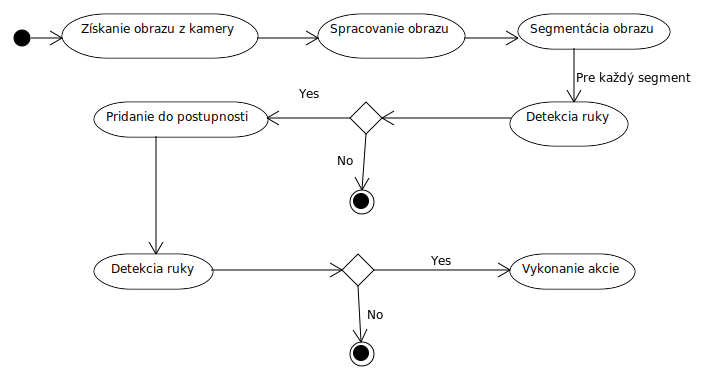
\includegraphics[width=\textwidth]{images/BaseAlgorithm}
%    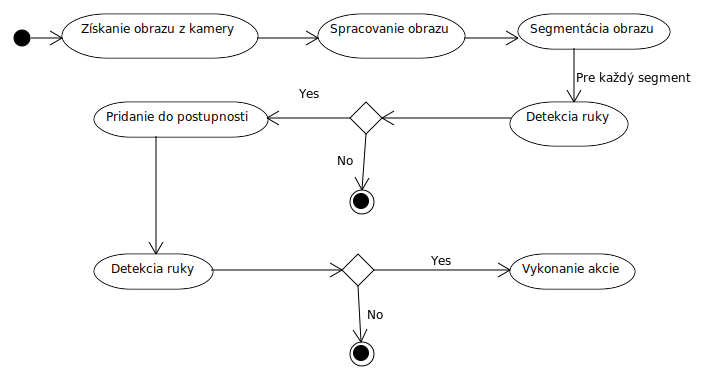
\includegraphics[scale=1]{images/BaseAlgorithm}
    \label{fig:base_alg}
    \caption{Základný algoritmus}
\end{figure}



